\documentclass[tikz,border=2pt]{standalone}
\usepackage{amsmath}
\usepackage{pgfplots}
\pgfplotsset{compat=1.18}
\usepgfplotslibrary{fillbetween}

\begin{document}
% In the (u,v)-plane a curve from (u1,v1) to (u2,v2): the area to its left (∫u dv) plus the
% area below it (∫v du) make up the rectangle u2 v2 minus the small rectangle u1 v1.
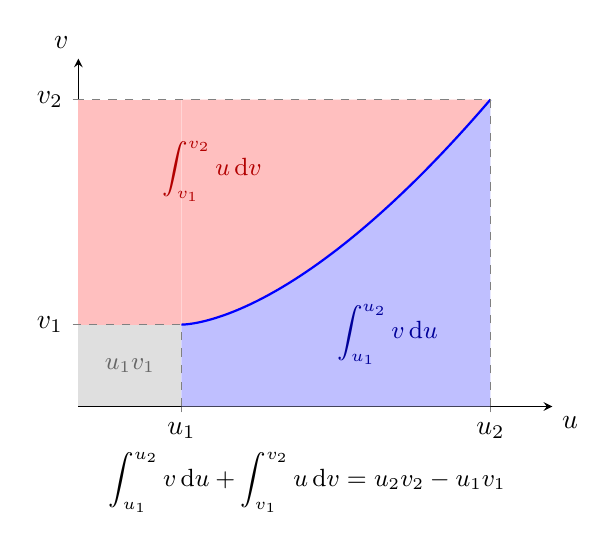
\begin{tikzpicture}
	\begin{axis}[
		axis lines=middle,
		xmin=0, xmax=4.6,
		ymin=0, ymax=3.4,
		xtick={1,4}, xticklabels={$u_1$,$u_2$},
		ytick={0.8,3}, yticklabels={$v_1$,$v_2$},
		xlabel={$u$}, ylabel={$v$},
		xlabel style={below right}, ylabel style={above left},
		samples=100, smooth, clip=false,
		width=7.6cm, height=6cm
		]
		% curve v = 0.8 + 2.2*((u-1)/3)^1.6 from (1,0.8) to (4,3)
		\addplot[name path=c, thick, blue, domain=1:4] {0.8+2.2*((x-1)/3)^1.6};
		\addplot[name path=top, draw=none, domain=1:4] {3};
		\addplot[name path=bottom, draw=none, domain=1:4] {0};
		\addplot[red!25] fill between[of=c and top];
		\addplot[blue!25] fill between[of=c and bottom];
		\fill[gray!25] (axis cs:0,0) rectangle (axis cs:1,0.8);
		\fill[red!25] (axis cs:0,0.8) rectangle (axis cs:1,3);
		\draw[dashed, gray] (axis cs:4,0) -- (axis cs:4,3) -- (axis cs:0,3);
		\draw[dashed, gray] (axis cs:1,0) -- (axis cs:1,0.8) -- (axis cs:0,0.8);
		\node[red!70!black, font=\small] at (axis cs:1.3,2.3) {$\displaystyle\int_{v_1}^{v_2}u\,\mathrm{d}v$};
		\node[blue!60!black, font=\small] at (axis cs:3.0,0.7) {$\displaystyle\int_{u_1}^{u_2}v\,\mathrm{d}u$};
		\node[gray!80!black, font=\small] at (axis cs:0.5,0.4) {$u_1v_1$};
		\node[anchor=north west, font=\small] at (axis cs:0.2,-0.35) {$\displaystyle\int_{u_1}^{u_2}v\,\mathrm{d}u+\int_{v_1}^{v_2}u\,\mathrm{d}v=u_2v_2-u_1v_1$};
	\end{axis}
\end{tikzpicture}
\end{document}
